\documentclass[a4paper, ngerman]{scrartcl}
\usepackage[T1]{fontenc}
\usepackage[utf8]{inputenc}
\usepackage{lmodern, tikz, xcolor}
\usetikzlibrary{tikzmark}

\newcommand{\darrow}[2]{
	\draw[->, thick, red] 
	({pic cs:#1}) ++(-0.1cm, -0.2cm) |- ++(0,-0.5cm) -|  ([yshift=-0.2cm, xshift=-0.1cm] {pic cs:#2});
}

\newcommand{\uarrow}[2]{
	\draw[->, thick, red] 
	({pic cs:#1}) ++(-0.1cm,0.4cm) |- ++(0,0.5cm) -|  ([yshift=0.4cm, xshift=-0.1cm] {pic cs:#2});
}

\definecolor{arrowColor1}{RGB}{0, 0, 255}     % Blue
\definecolor{arrowColor2}{RGB}{0, 128, 0}     % Dark Green
\definecolor{arrowColor3}{RGB}{0, 170, 0}     % Dark Green
\definecolor{arrowColor4}{RGB}{128, 0, 128}   % Purple
\definecolor{arrowColor5}{RGB}{0, 255, 255}   % Cyan
\definecolor{arrowColor6}{RGB}{255, 105, 180}  % Hot Pink
\definecolor{arrowColor7}{RGB}{255, 192, 203} % Light Pink
\definecolor{arrowColor8}{RGB}{255, 200, 200}    % Gold

\begin{document}
	
	\begin{figure}[htbp]
		\begin{tabular}{|c|c|c|c|c|c|c|c|c|c|c|c|c|c|c|c|c|c|c|}
			\hline
			\multicolumn{2}{|r|}{Ciphertext} & S & N\tikzmark{end1} & M & K & G\tikzmark{end4} & G\tikzmark{start5} & S\tikzmark{start6} & T & Z & Z & U\tikzmark{start10} & G & A\tikzmark{start12} & R & L & V\tikzmark{start15}\\
			\hline
			\multicolumn{2}{|r|}{Crib} & W & E\tikzmark{start1} & T & T & E\tikzmark{start4} & R\tikzmark{end5} & V\tikzmark{end6} & O & R & H & E\tikzmark{end10} & R & S\tikzmark{end12} & A & G & E\tikzmark{end15}\\
			\hline
		\end{tabular}
		
		\begin{tikzpicture}[remember picture, overlay]
			\draw[->, thick, blue] 
			({pic cs:start10}) ++(-0.1cm, 1.4cm) |- ++(0, -0.5cm) -| ([yshift=0.4cm, xshift=-0.1cm] {pic cs:start10});
			
			\draw[->, thick, arrowColor1] 
			({pic cs:end10}) ++(-0.1cm, -0.2cm) |- ++(0,-0.5cm) -|  ([yshift=-0.2cm, xshift=-0.1cm] {pic cs:start4});
			
			\draw[->, thick, arrowColor2] 
			({pic cs:end4}) ++(-0.1cm,0.4cm) |- ++(0,0.5cm) -|  ([yshift=0.4cm, xshift=-0.1cm] {pic cs:start5});
			
			\draw[->, thick, arrowColor3] ({pic cs:end5}) ++(-0.1cm,-0.2cm) |- ++(0.2cm,-0.3cm) |- ++(0,1.9cm) -|  ([yshift=0.4cm, xshift=-0.1cm]{pic cs:start12});
			
			\draw[->, thick, arrowColor4] ({pic cs:end12}) ++(-0.1cm,-0.2cm) |- ++(-0.2cm,-0.3cm) |- ++(0,1.75cm) -|  ([yshift=0.45cm, xshift=-0.1cm]{pic cs:start6});
			
			\draw[->, thick, red] ({pic cs:end6}) ++(-0.1cm,-0.2cm) |- ++(0.2cm,-0.3cm) |- ++(0,1.6cm) -|  ([yshift=0.45cm, xshift=-0.1cm]{pic cs:start15});
			
			\draw[->, thick, red] 
			({pic cs:end15}) ++(-0.1cm, -0.2cm) |- ++(0,-0.5cm) -|  ([yshift=-0.2cm, xshift=0.05cm] {pic cs:end10});
		\end{tikzpicture}
	\end{figure}
	
\end{document}